% -------------------------------------------------------------------------------------------------------
%-----------------------------CONSULTA DE PROGRAMAS ACADÉMICOS---------------------------------
% -------------------------------------------------------------------------------------------------------
\section{Gestión de Programas Académicos}
    \subsection{Consulta de Programas Académicos}
        Cuando el usuario da clic en la sección de \textbf{Gestionar Programas Académicos} se muestra la pantalla:
        \begin{figure}[H]
        	\centering
        	\hypertarget{consultarpa}{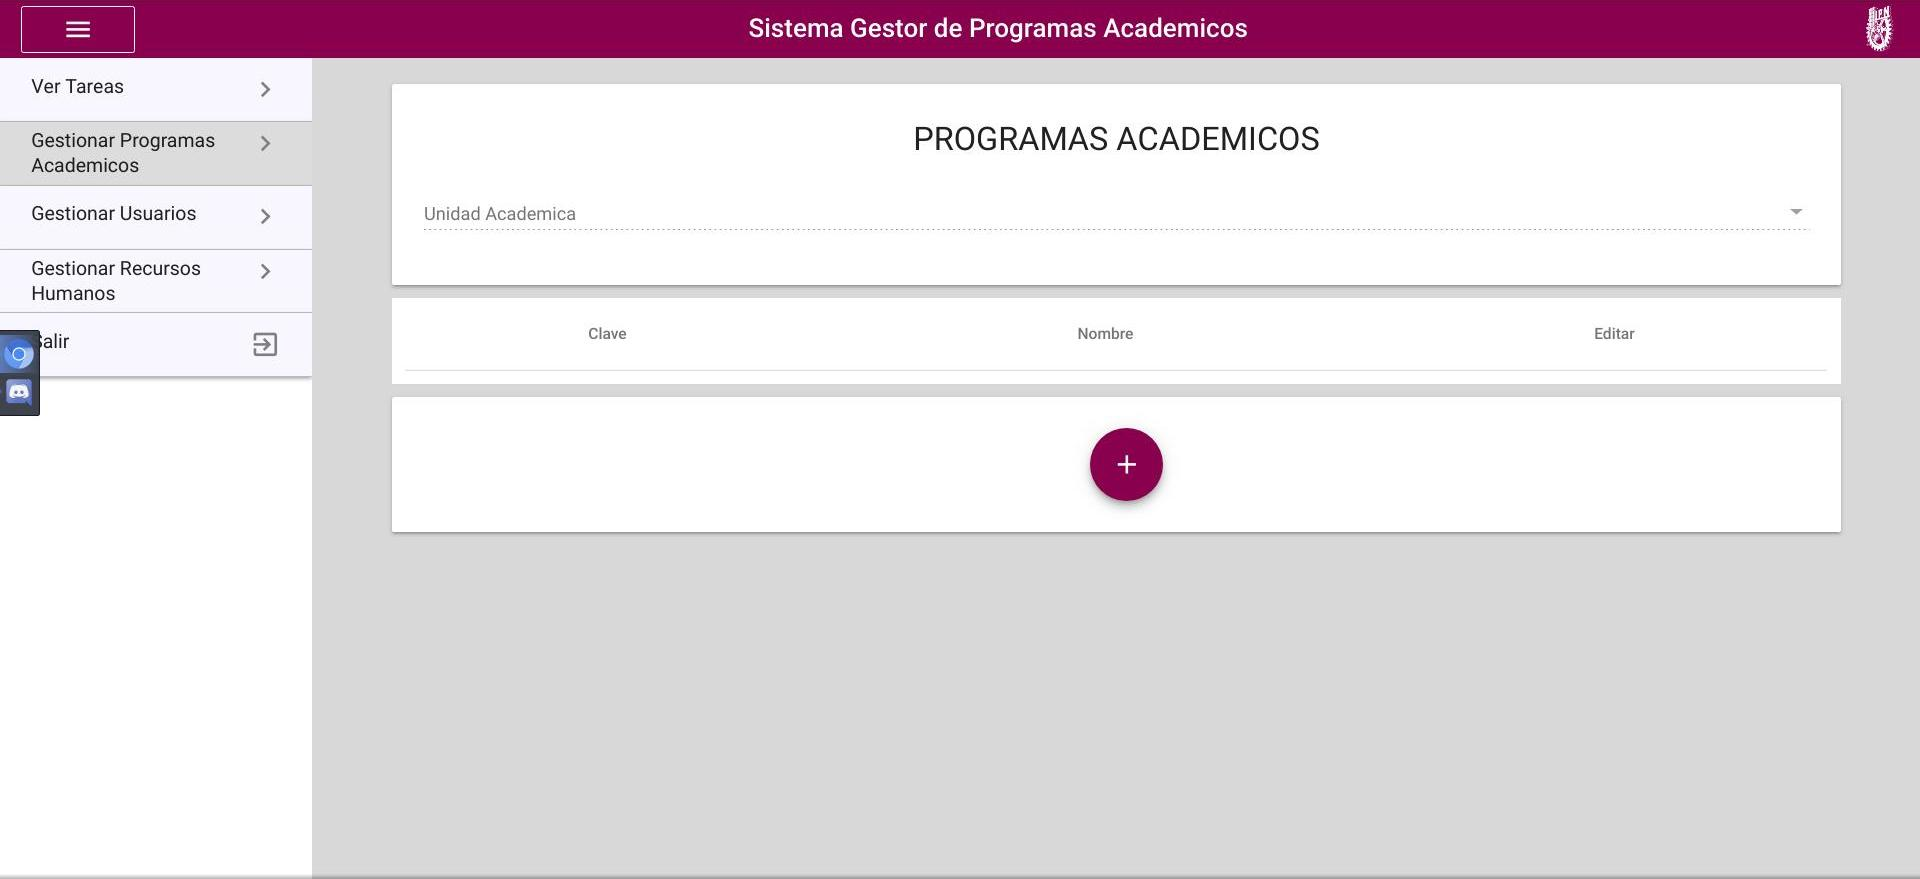
\includegraphics[width=0.7\linewidth]{images/SP3/ConsultarPA}}
        	\caption{Pantalla para Gestionar Programas Académicos}
        	\label{consultarpa}
        \end{figure}

        En donde aparece, de forma predeterminada, todos los Programas Académicos  registrados en el sistema al momento de su Unidad Académica. Tiene a su disposición 2 funciones:

	    \subsection{Editar Programa Académico}

        	Para ello, el usuario da clic en el botón \BtnLapiz que esta junto al Programa Académico que desea modificar. Al hacer esto, se le redirecciona a la pantalla de \hyperlink{editarpa}{\textit{Editar Programa Académico}}.
        	\begin{figure}[H]
        		\centering
        		\hypertarget{editar}{
\includegraphics[width=0.7\linewidth]{images/SP3/BtnEditar}}
        		\caption{Botón Editar Programa Académico}
        		\label{editar}
        	\end{figure}
        \begin{figure}[H]
        	\centering
        	\hypertarget{editarpa}{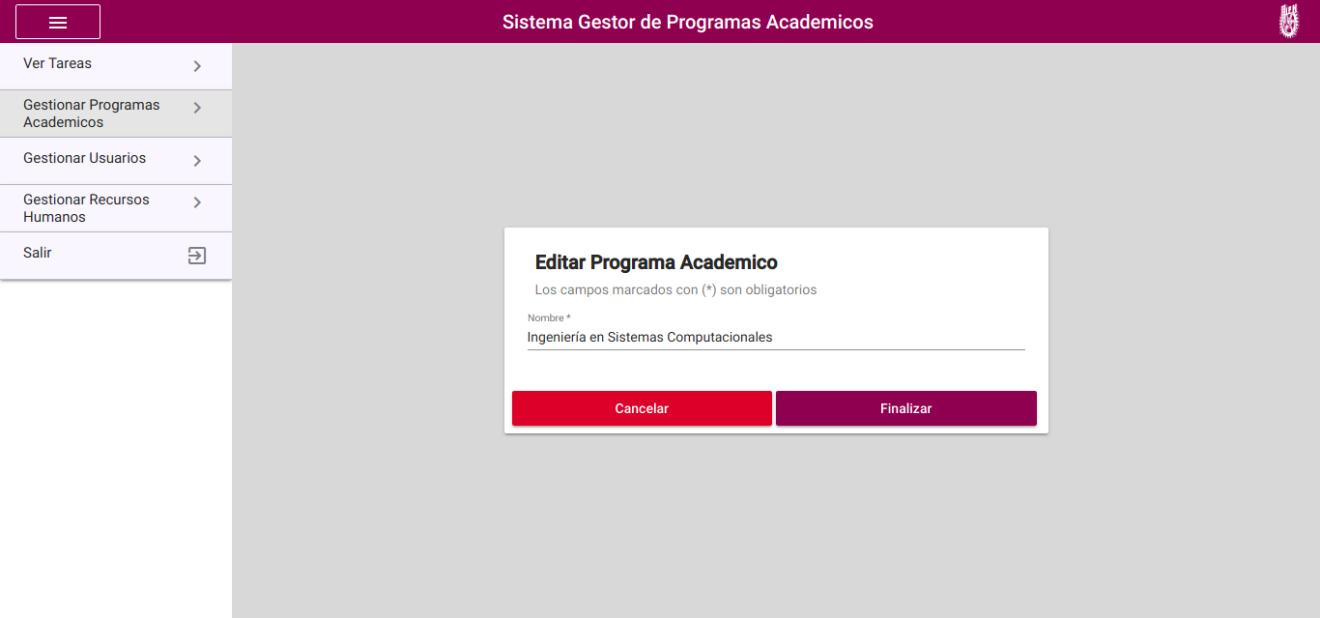
\includegraphics[width=0.7\linewidth]{images/SP3/EditarPA}}
        	\caption{Pantalla para la edición de Programas Académicos}
        	\label{editarpa}
        \end{figure}

        En donde se cargan los datos del Programa Académico seleccionado en la pantalla de \hyperlink{consultarpa}{\textit{Consultar Programas Académicos}} y se llena el formulario.\\

        El usuario puede modificar todos los campos del Programa Académico:
        \begin{figure}[H]
        	\centering
        	\hypertarget{modif}{
\includegraphics[width=0.7\linewidth]{images/SP3/Editado}}
        	\caption{Datos del Programa Académico modificados}
        	\label{modif}
        \end{figure}

        Si el usuario da clic en el botón \IUbutton{Cancelar}:

        \begin{figure}[H]
        	\centering
        	\hypertarget{cancel2}{
\includegraphics[width=0.7\linewidth]{images/SP3/BtnCancelar}}
        	\caption{Botón ''Cancelar''}
        	\label{cancel2}
        \end{figure}

       Se muestra el siguiente mensaje:
        %Imagen MSG29
        \begin{figure}[H]
            \centering
            \hypertarget{confirmar}{
\includegraphics[width=0.7\linewidth]{images/SP3/Confirmacion}}
            \caption{Confirmación}
            \label{confirmar}
        \end{figure}

        Para confirmar, el usuario da clic al botón \IUbutton{Sí}, y el Programa Académico no es modificado.\\

        Si el usuario da clic al botón \IUbutton{No}, el mensaje se cierra y el usuario continúa con la edición del Programa Académico.\\

        Cuando el usuario da clic al botón \IUbutton{Finalizar}.
        \begin{figure}[H]
        	\centering
        	\hypertarget{btnfin}{
\includegraphics[width=0.7\linewidth]{images/SP3/BtnFinalizar}}
        	\caption{Botón ''Finalizar''}
        	\label{btnfin}
        \end{figure}

        Si no ocurrieron errores, el sistema muestra el siguiente mensaje:

        \begin{figure}[H]
            \centering
            \hypertarget{cambio}{
\includegraphics[width=0.7\linewidth]{images/SP3/Cambio}}
            \caption{Cambio exitoso.}
            \label{cambio}
        \end{figure}

        Si da clic sobre el botón \IUbutton{Aceptar}, se le redirecciona a la pantalla de \hyperlink{consultarpa}{\textit{Gestionar Programas Académicos}}, en donde verá las modificaciones al Programa Académico.\\

        \subsubsection{Posibles errores}

            \begin{itemize}
            	\item Campos vacíos al momento de modificar el Programa Académico

                	Si el usuario deja en blanco algún campo del formulario, aparece el siguiente mensaje:

                    \begin{figure}[H]
                    \centering
                    \hypertarget{vacio}{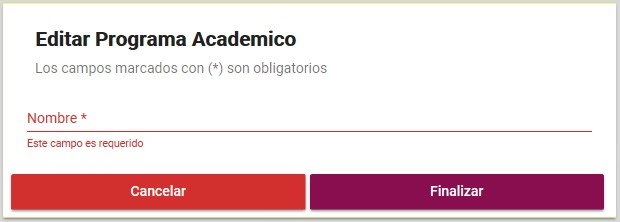
\includegraphics[width=0.7\linewidth]{images/SP3/Vacio}}
                    \caption{Campo Vacío}
                    \label{vacio}
                    \end{figure}

            	\item Los campos ingresados no son válidos

                	Si al momento de ingresar los datos aparece el siguiente mensaje:

                     \begin{figure}[H]
                    \centering
                    \hypertarget{invalido}{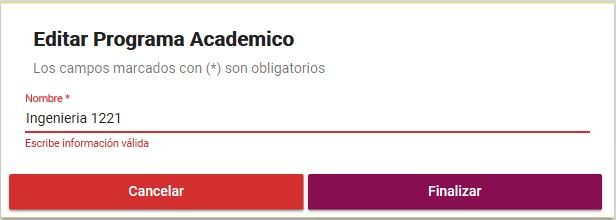
\includegraphics[width=0.7\linewidth]{images/SP3/Invalida}}
                    \caption{Campo invalido}
                    \label{invalido}
                    \end{figure}


                	Significa que la composición de los datos ingresados en el formulario no es la correcta. Tenga en cuenta lo siguiente:

                	\begin{itemize}
                		\item El nombre se compone  únicamente de letras y espacios.

                        \item El nombre tiene una longitud máxima de 150 carácteres.
                	\end{itemize}

                \item El nombre del Programa Académico ya está registrado.
                    Si al momento de Finalizar la Edición se muestra este mensaje.

                     \begin{figure}[H]
                    \centering
                    \hypertarget{vacio}{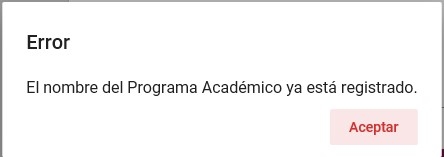
\includegraphics[width=0.7\linewidth]{images/SP3/Yareg}}
                    \caption{Campo Vacío}
                    \label{vacio}
                    \end{figure}

                    Significa que el Programa Académico ya ha sido registrado previamente dentro de la Unidad Académica.



            \end{itemize}
        \subsection{Registrar Programa Académico}

            El usuario debe dar clic en el botón \IUbutton{+} en la parte inferior de la pantalla.

            \begin{figure}[H]
                \centering
                \hypertarget{add}{
\includegraphics[width=0.7\linewidth]{images/SP3/BtnAgregar}}
                \caption{Botón Agregar Programa Académico}
                \label{add}
            \end{figure}

            Al hacerlo, es redireccionado a la pantalla de \hyperlink{registrarpa}{\textit{Registrar Programa Académico}}.

        \begin{figure}[H]
            \centering
            \hypertarget{registrarpa}{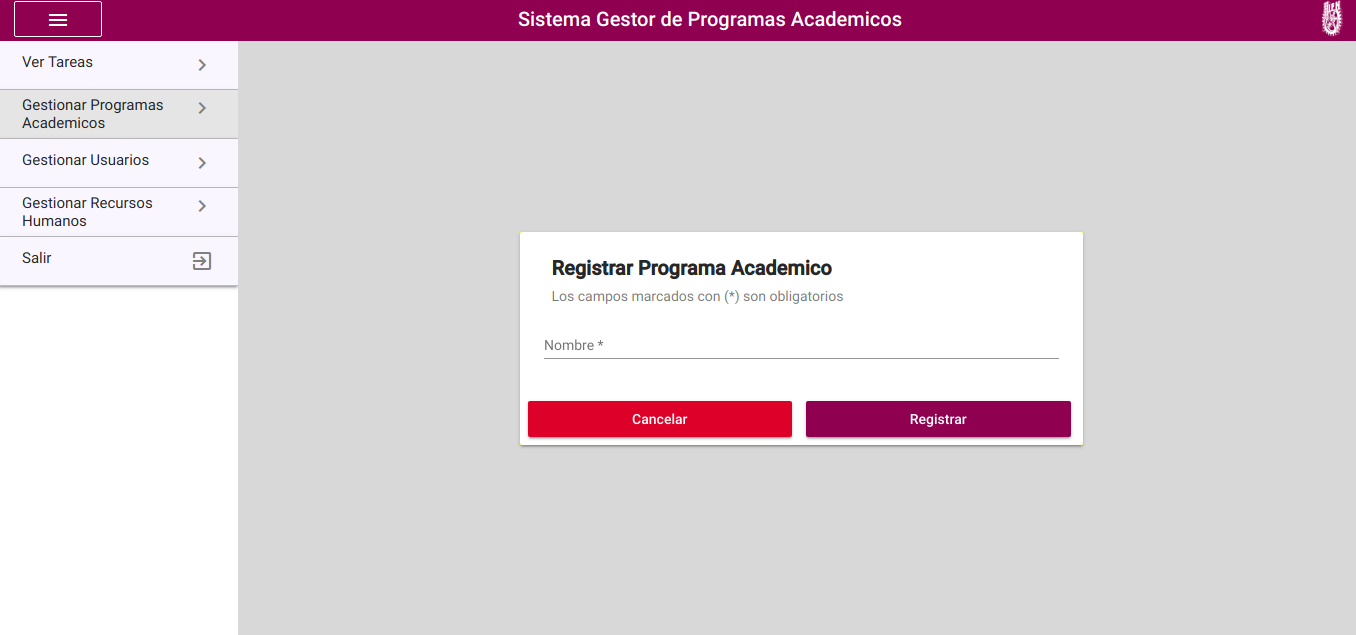
\includegraphics[width=0.7\linewidth]{images/SP3/RegistrarPA}}
            \caption{Pantalla para registrar Programas Académicos}
            \label{registrarpa}
        \end{figure}

        En donde ingresa los datos del nuevo Programa Académico en el formulario. Un ejemplo del llenado sería el siguiente:

        \begin{figure}[H]
            \centering
            \hypertarget{ejreg}{
\includegraphics[width=0.7\linewidth]{images/SP3/Llenado}}
            \caption{Ejemplo de llenado para agregar un nuevo Programa Académico}
            \label{ejreg}
        \end{figure}

        Si el usuario da clic en el botón \IUbutton{Cancelar}:

        \begin{figure}[H]
            \centering
            \hypertarget{cancel1}{
\includegraphics[width=0.7\linewidth]{images/SP3/BtnCancelar}}
            \caption{Botón ''Cancelar''}
            \label{cancel1}
        \end{figure}

         Se muestra el siguiente mensaje:

        \begin{figure}[H]
            \centering
            \hypertarget{confirmar}{
\includegraphics[width=0.7\linewidth]{images/SP3/Confirmacion}}
            \caption{Confirmación}
            \label{confirmar}
        \end{figure}

        Para confirmar, el usuario da clic al botón \IUbutton{Sí}, y el Programa Académico no es registrado.\\

        Para cancelar, el usuario da clic al botón \IUbutton{No}, el mensaje se cierra y el usuario continúa en el formulario.\\

        A continuación, una vez verificados los datos, deberá de dar clic al botón \IUbutton{Registrar}.
        \begin{figure}[H]
            \centering
            \hypertarget{btnreg}{
\includegraphics[width=0.7\linewidth]{images/SP3/BtnRegistrar}}
            \caption{Botón ''Registrar''}
            \label{btnreg}
        \end{figure}

        Si no ocurrieron errores, se muestra el siguiente mensaje:

        \begin{figure}[H]
            \centering
            \hypertarget{exito}{
\includegraphics[width=0.7\linewidth]{images/SP3/Exitoso}}
            \caption{Registo exitoso.}
            \label{exito}
        \end{figure}

        Cuando da clic al botón \IUbutton{Aceptar}, se le redirecciona a la pantalla de \hyperlink{consultarpa}{\textit{Gestionar Programas Académicos}}, en donde ve el nuevo Programa Académico agregado.\\


        \subsubsection{Posibles errores}

            \begin{itemize}
                \item Campos vacíos al momento de modificar el Programa Académico

                    Si el usuario deja en blanco algún campo del formulario, aparece el siguiente mensaje:

                    \begin{figure}[H]
                    \centering
                    \hypertarget{vacio}{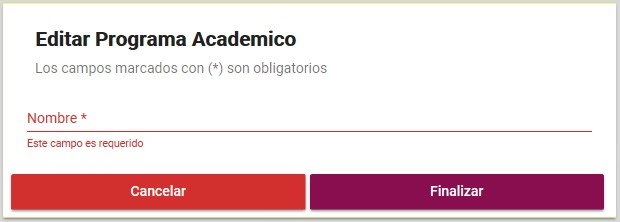
\includegraphics[width=0.7\linewidth]{images/SP3/Vacio}}
                    \caption{Campo Vacío}
                    \label{vacio}
                    \end{figure}

                \item Los campos ingresados no son válidos

                    Si al momento de ingresar los datos aparece el siguiente mensaje:

                     \begin{figure}[H]
                    \centering
                    \hypertarget{invalido}{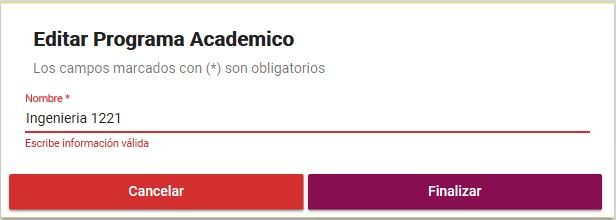
\includegraphics[width=0.7\linewidth]{images/SP3/Invalida}}
                    \caption{Campo invalido}
                    \label{invalido}
                    \end{figure}


                    Significa que la composición de los datos ingresados en el formulario no es la correcta. Tenga en cuenta lo siguiente:

                    \begin{itemize}
                        \item El nombre se compone únicamente de letras y espacios.

                        \item El nombre tiene una longitud máxima de 150 carácteres.
                    \end{itemize}

                \item El nombre del Programa Académico ya está registrado.
                    Si al momento de Finalizar el Registro se muestra este mensaje:

                     \begin{figure}[H]
                    \centering
                    \hypertarget{vacio}{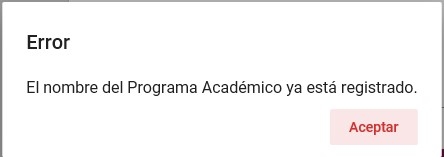
\includegraphics[width=0.7\linewidth]{images/SP3/Yareg}}
                    \caption{Campo Vacío}
                    \label{vacio}
                    \end{figure}

                    Significa que el Programa Académico ya ha sido registrado previamente dentro de la Unidad Académica.
            \end{itemize}
